\section{Presentazioni}
\begin{frame}\centering
  \frametitle{La classe Beamer}
  \texttt{\textbackslash{}documentclass[aspectratio=169]\{beamer\} \% prima riga}
  \pause
  \texttt{\\\dots\\
  \textbackslash{}begin\{frame\} \%dentro il document
\\
  ~~\textbackslash{}frametitle\{Titolo\}~~~~~~~~~~~~~
\\
  ~~\textbackslash{}framesubtitle\{Sottotitolo\}~~~~~
\\
  \textbackslash{}end\{frame\}
~~~~~~~~~~~~~~~~~~~~~~~\\~}
\end{frame}
\begin{frame}\centering
  \frametitle{Comandi noti}
  Preambolo: codifica dei caratteri, pacchetti da includere, \dots\\~\\\pause
  Titolo: \texttt{\textbackslash{}maketitle}\\~\\\pause
  \texttt{\textbackslash{}section, \textbackslash{}subsection}\\~\\\pause
  Formattazione testo, immagini, note a piè di pagina, bibliografia, \dots
\end{frame}
\begin{frame}\centering
  \frametitle{Indice}
  \texttt{~\\
  \textbackslash{}begin\{frame\}~~~~~~~~~~~\\
  ~~\textbackslash{}frametitle\{Contenuti\}\\
  ~~\textbackslash{}tableofcontents~~~~~~~~\\
  \textbackslash{}end\{frame\}~~~~~~~~~~~~~\\~
}
\end{frame}
\begin{frame}\centering
  \frametitle{Animazioni}
  \texttt{Questa è \textbackslash{}pause una prova}\\~\\\pause
  Questa è \pause una prova
\end{frame}
\begin{frame}\centering
\frametitle{Temi e colori}
  \begin{tabular}{ll}
    \texttt{\textbackslash{}usetheme\{Warsaw\}}&\only<2->{Esempi di tutte le combinazioni tema-colore: }\\
    \texttt{\textbackslash{}usecolortheme\{seahorse\}} & \only<2->{\url{https://hartwork.org/beamer-theme-matrix/}}
  \end{tabular}
  \visible<2->{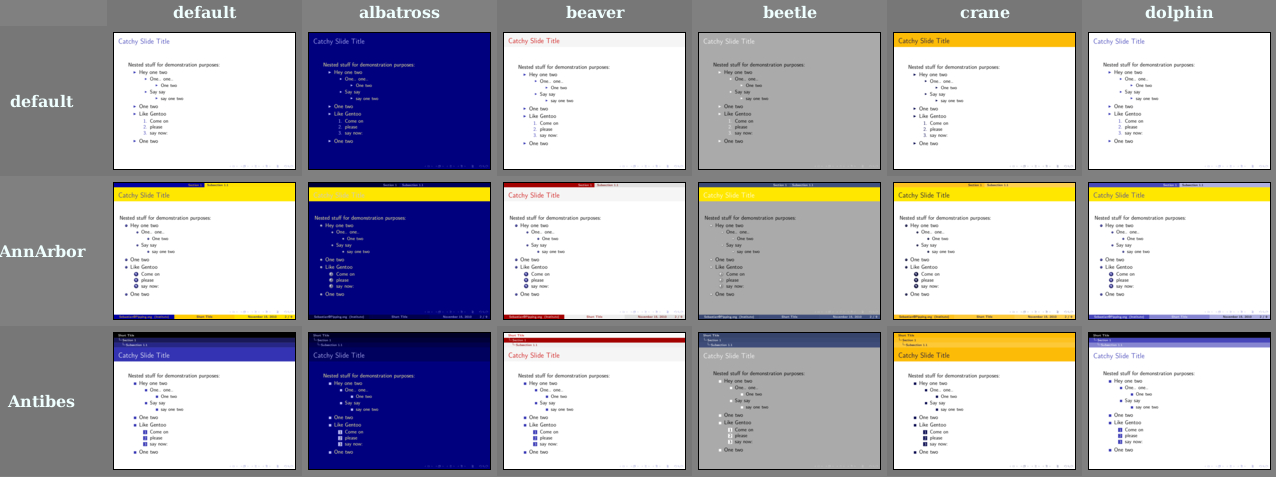
\includegraphics[width=400px]{img/beamer_beamer}}
\end{frame}

